\section{Exercise 1b: Envelope Detection}
\label{sec:ex1b}

\subsection*{Objective}
Implement an envelope detector using rectification and low-pass filtering, then compare it with coherent detection.

\subsection*{Module Design}
The envelope detection sub-VI is shown in Figure~\ref{fig:envelope_vi}.
\begin{figure}[H]
\centering
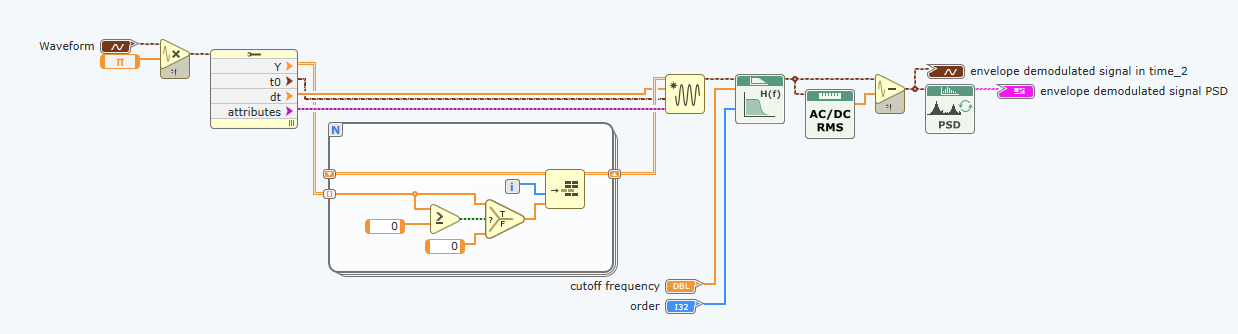
\includegraphics[width=\linewidth]{figures/Envelope_Devodulation_VI.png}
\caption{Block diagram of the envelope detection VI.}
\label{fig:envelope_vi}
\end{figure}

The implemented signal flow is:
\begin{enumerate}
\item Apply a pre-gain of $\pi$ to compensate rectification loss.
\item Convert waveform data to array form.
\item Perform half-wave rectification (negative samples set to zero) in a loop.
\item Rebuild the waveform while preserving timing information ($t_0$ and $dt$).
\item Apply a Butterworth low-pass filter.
\item Remove the DC component and estimate the PSD of the recovered signal.
\end{enumerate}

\subsection*{Link to Theory}
Envelope detection is a nonlinear approximation to message recovery. It works by extracting slow envelope variation and rejecting carrier ripple through low-pass filtering. The method is valid when the envelope does not invert, i.e.
\begin{equation}
\mu \le 1.
\end{equation}
For $\mu > 1$, over-modulation causes envelope inversion and strong distortion in the recovered signal.

The $\pi$ pre-gain compensates the dominant amplitude loss introduced by half-wave rectification, consistent with the rectification-loss analysis in the handout appendix.

\subsection*{Implementation Notes}
\begin{itemize}
\item Preserving waveform timing during array conversion/rebuild is essential; otherwise the recovered frequency axis becomes incorrect.
\item The same low-pass design logic as coherent detection is used: pass message bandwidth, reject carrier-related components.
\item DC removal is required because the detected envelope contains a large mean term linked to the carrier.
\end{itemize}

\subsection*{Expected Output}
For $\mu \le 1$, the time-domain output tracks the message envelope and PSD shows the message component near $f_m$. As $\mu$ exceeds 1, visible distortion appears even after filtering.
